\documentclass[border=2pt]{standalone}
\usepackage[dvipsnames,svgnames,x11names]{xcolor}
\usepackage{tikz}
\usetikzlibrary{arrows.meta,positioning}
\begin{document}
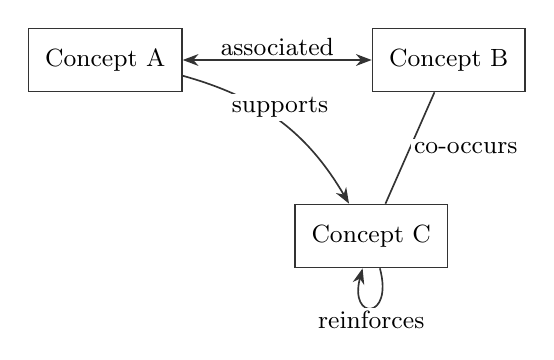
\begin{tikzpicture}[font=\small,>=Stealth]
\node[rectangle,fill=white,draw=black!80,text=black,line width=0.6pt,minimum height=8mm,inner xsep=6pt,inner ysep=4pt,align=center] (a) at (0,0) {Concept A};
\node[rectangle,fill=white,draw=black!80,text=black,line width=0.6pt,minimum height=8mm,inner xsep=6pt,inner ysep=4pt,align=center,right=24mm of a] (b) {Concept B};
\node[rectangle,fill=white,draw=black!80,text=black,line width=0.6pt,minimum height=8mm,inner xsep=6pt,inner ysep=4pt,align=center,below right=20mm of a] (c) {Concept C};
\draw[<->,draw=black!80,line width=0.6pt] (a) -- node[pos=0.5,above,fill=white,inner sep=1.2pt] {associated} (b);
\draw[->,draw=black!80,line width=0.6pt] (a) to[bend left=22] node[pos=0.5,above,fill=white,inner sep=1.2pt] {supports} (c);
\draw[-,draw=black!80,line width=0.6pt] (b) -- node[pos=0.5,right,fill=white,inner sep=1.2pt] {co-occurs} (c);
\draw[->,draw=black!80,line width=0.6pt] (c) to[loop below] node[pos=0.5,below,fill=white,inner sep=1.2pt] {reinforces} (c);
\end{tikzpicture}
\end{document}
